\documentclass[12pt,a4paper,bibliography=totocnumbered,listof=totocnumbered]{scrartcl}
\usepackage[ngerman]{babel}
\usepackage[utf8]{inputenc}
\usepackage{amsmath}
\usepackage{amsfonts}
\usepackage{amssymb}
\usepackage{graphicx}
\usepackage{fancyhdr}
\usepackage{tabularx}
\usepackage{geometry}
\usepackage{setspace}
\usepackage[right]{eurosym}
\usepackage[printonlyused]{acronym}
\usepackage{subfig}
\usepackage{floatflt}
\usepackage[usenames,dvipsnames]{color}
\usepackage{colortbl}
\usepackage{paralist}
\usepackage{array}
\usepackage{titlesec}
\usepackage{parskip}
\usepackage[right]{eurosym}
\usepackage{picins}
\usepackage[subfigure,titles]{tocloft}
\usepackage[pdfpagelabels=true]{hyperref}
\usepackage{listings}

\usepackage{color}

% \lstset{basicstyle=\footnotesize, captionpos=b, breaklines=true, showstringspaces=false, tabsize=2, frame=lines, numbers=left, numberstyle=\tiny, xleftmargin=2em, framexleftmargin=2em}
% \makeatletter
% \def\l@lstlisting#1#2{\@dottedtocline{1}{0em}{1em}{\hspace{1,5em} Lst. #1}{#2}}
% \makeatother

\geometry{a4paper, top=27mm, left=30mm, right=20mm, bottom=35mm, headsep=10mm, footskip=12mm}

% \hypersetup{unicode=false, pdftoolbar=true, pdfmenubar=true, pdffitwindow=false, pdfstartview={FitH},
% 	pdftitle={Abschlussarbeit},
% 	pdfauthor={Daniel Brettschneider},
% 	pdfsubject={Abschlussarbeit},
% 	pdfcreator={\LaTeX\ with package \flqq hyperref\frqq},
% 	pdfproducer={pdfTeX \the\pdftexversion.\pdftexrevision},
% 	pdfkeywords={Abschlussarbeit},
% 	pdfnewwindow=true,
% 	colorlinks=true,linkcolor=black,citecolor=black,filecolor=magenta,urlcolor=black}
% \pdfinfo{/CreationDate (D:20110620133321)}

\begin{document}

\titlespacing{\section}{0pt}{12pt plus 4pt minus 2pt}{-6pt plus 2pt minus 2pt}

% Kopf- und Fusszeile
\renewcommand{\sectionmark}[1]{\markright{#1}}
\renewcommand{\leftmark}{\rightmark}
\pagestyle{fancy}
\lhead{}
\chead{}
\rhead{\thesection\space\contentsname}
\lfoot{Ausblick}
\cfoot{}
\rfoot{\ \linebreak Seite \thepage}
\renewcommand{\headrulewidth}{0.4pt}
\renewcommand{\footrulewidth}{0.4pt}

% Vorspann
\renewcommand{\thesection}{\arabic{section}}
\renewcommand{\theHsection}{\arabic{section}}
\pagenumbering{arabic}

% ----------------------------------------------------------------------------------------------------------
% Titelseite
% ----------------------------------------------------------------------------------------------------------
\thispagestyle{empty}
\begin{center}
	
\includegraphics[scale=1]{Bilder/uni_os_l.png}\\
	\vspace*{2cm}
	\Large
	\textbf{Fachbereich}\\
	\textbf{Humanwissenschaften}\\
	\textbf{Institut für Cognitive Science}\\
	\vspace*{2cm}
	\Huge
	\textbf{Bachelorarbeit - Ausblick}\\
	\vspace*{0.5cm}
	\large
	Automatisierte Analyse von Preisbildungsmustern\\
	anhand von Zeitreihendaten der Markttransparenzstelle für Kraftstoffe\\
	% \vspace*{1cm}
	% \textbf{Ausblick}\\
	\vspace*{2cm}
	
	\vfill
	\normalsize
	\newcolumntype{x}[1]{>{\raggedleft\arraybackslash\hspace{0pt}}p{#1}}
	\begin{tabular}{x{6cm}p{7.5cm}}
		\rule{0mm}{5ex}\textbf{Autor:} & Kai Fritsch\newline kai.m.fritsch@gmail.com \\ 
		\rule{0mm}{5ex}\textbf{Prüfer:} & Prof. Dr. Oliver Vornberger \\ 
		% \rule{0mm}{5ex}\textbf{Abgabedatum:} & - \\ 
	\end{tabular} 
\end{center}
\pagebreak

% ----------------------------------------------------------------------------------------------------------
% Abstract
% ----------------------------------------------------------------------------------------------------------
\setcounter{page}{1}
\onehalfspacing
\titlespacing{\section}{0pt}{12pt plus 4pt minus 2pt}{2pt plus 2pt minus 2pt}
\rhead{Ausblick}
\section{Motivation}
Kraftstoffpreise unterliegen seid je her großen Preisschwankungen. Die hohe Homogenität und sinkende Nachfrage sind optimale Bedingungen für starken Konkurenzdruck. Der Druck ist so hoch, dass die Anzahl an Tankstellen in Deutschland seit 1970 von gut 46.000 auf heute knapp 15.000 gefallen ist.\cite{PraTa} Nichts desto trotz ist die Anzahl an Preisänderungen in den letzten Jahren noch einmal merklich gestiegen. Während der Preis 2011 noch durchschnittlich weniger als zwei mal pro Tag geändert wurde, sind die meisten Tankstellen inzwischen bei um die sechs Änderungen pro Tag angelangt.\cite{Unity} Mitgrund für diese jüngste Steigerung könnten diesmal jedoch die neuerlichen elektronische Möglichkeiten sein.\\

Während Tankstelleninhaber vor einigen Jahren noch ihre Konkurenz einen Besuch abstatten mussten um deren Preise auszukundschaften, reicht heutzutage eine Suchanfrage im Netz. Und selbst diese ist seit der Einführung der Markttransparenzstelle für Kraftstoffe nicht mehr notwendig. Jede Tankstelle ist seit Ende 2013 verpflichtet ihre Preisänderungen dem Bundeskartelamt für Kraftsotffe elektronisch zu übermitteln. Die live Verfügbarkeit aller aktuellen Preise ermöglicht es Tankstellenbesitzern mittels bestimmter Programme ihre Preise vollautomatisch an die Konkurenz anzupassen. Der auf diese Weise enstandene Datensatz und die verbreitete Verwendung von automatisierten Preisführungstools (Pricing-Tools) bilden somit die Grundlagen dieser Arbeit.\\

Ziel dieser Arbeit soll es sein anhand der gesammelten Daten von grob zwei Jahren das Pricing Verhalten der einzelnen Tankstellen zu analysierten. Da  viele Tankstellen solche automatisch arbeitenden Tools verwenden liegt es nahe, dass sich in den Daten bestimmte Muster abzeichnen könnten, die Rückschlüsse über die zugrunde liegenden Regeln, dieser Tools zulassen könnten. Das Wissen um solche Regeln, würde es ermöglichen das Pricing Verhalten der Konkurenz genauer vorherzusagen und einem somit einen Vorteil im Wettbewerb verschaffen. Es könnte auch dabei helfen Rückschlüsse über die genauere Ursache der starken Schwankungen zu finden und somit eventuell Wege  aufzeigen um das allgemeine Preisverhalten wieder zu stabilisieren. 
\newpage
\vspace{-1,2em}

\titlespacing{\section}{0pt}{12pt plus 4pt minus 2pt}{-6pt plus 2pt minus 2pt}
\section{Grundlagen}
Um Muster überhaupt erkennen zu können, ist es notwendig sowohl das Medium in dem die Muster gesucht werden, als auch die möglichen Strukturen der Muster so gut wie möglich zu kennen. Deshalb werden im nächsten Abschnitt zum Einen der Datensatz der Markttransarenzstelle(MTS) für Kraftstoffe, sowie zum Anderen der exemplarische Aufbau eines der verwendeten Pricing-Tools beschrieben.

\titlespacing{\subsection}{0pt}{12pt plus 4pt minus 2pt}{-6pt plus 2pt minus 2pt}
\subsection{Datensatz}

\begin{quote} 
\glqq Seit dem 31. August 2013 sind Unternehmen, die öffentliche Tankstellen betreiben oder über die Preissetzungshoheit an diesen verfügen, verpflichtet, Preisänderungen bei den gängigen Kraftstoffsorten Super E5, Super E10 und Diesel in Echtzeit an die Markttransparenzstelle für Kraftstoffe zu melden.\grqq\cite{BkMTS}
\end{quote}

In Echtzeit bedeutet hier, dass die Information über eine Preisänderung spätestens 5 Minuten nach der Änderung selber an der MTS eingehen müssen. Neben den Preisänderungen müssen auch die Stammdaten der Tankstellen wöchentlich an die MTS gemeldet werden. Die MTS veröffentlicht die Daten jedoch nicht direkt selber sondern stellt die Daten Verbraucherinformationsdiensten(VID) zur Verfügung. Diesen verpflichten sich die Daten in irgendeiner Form den Verbrauchern als nützliche Information zukommen zu lassen. 

\begin{center}
	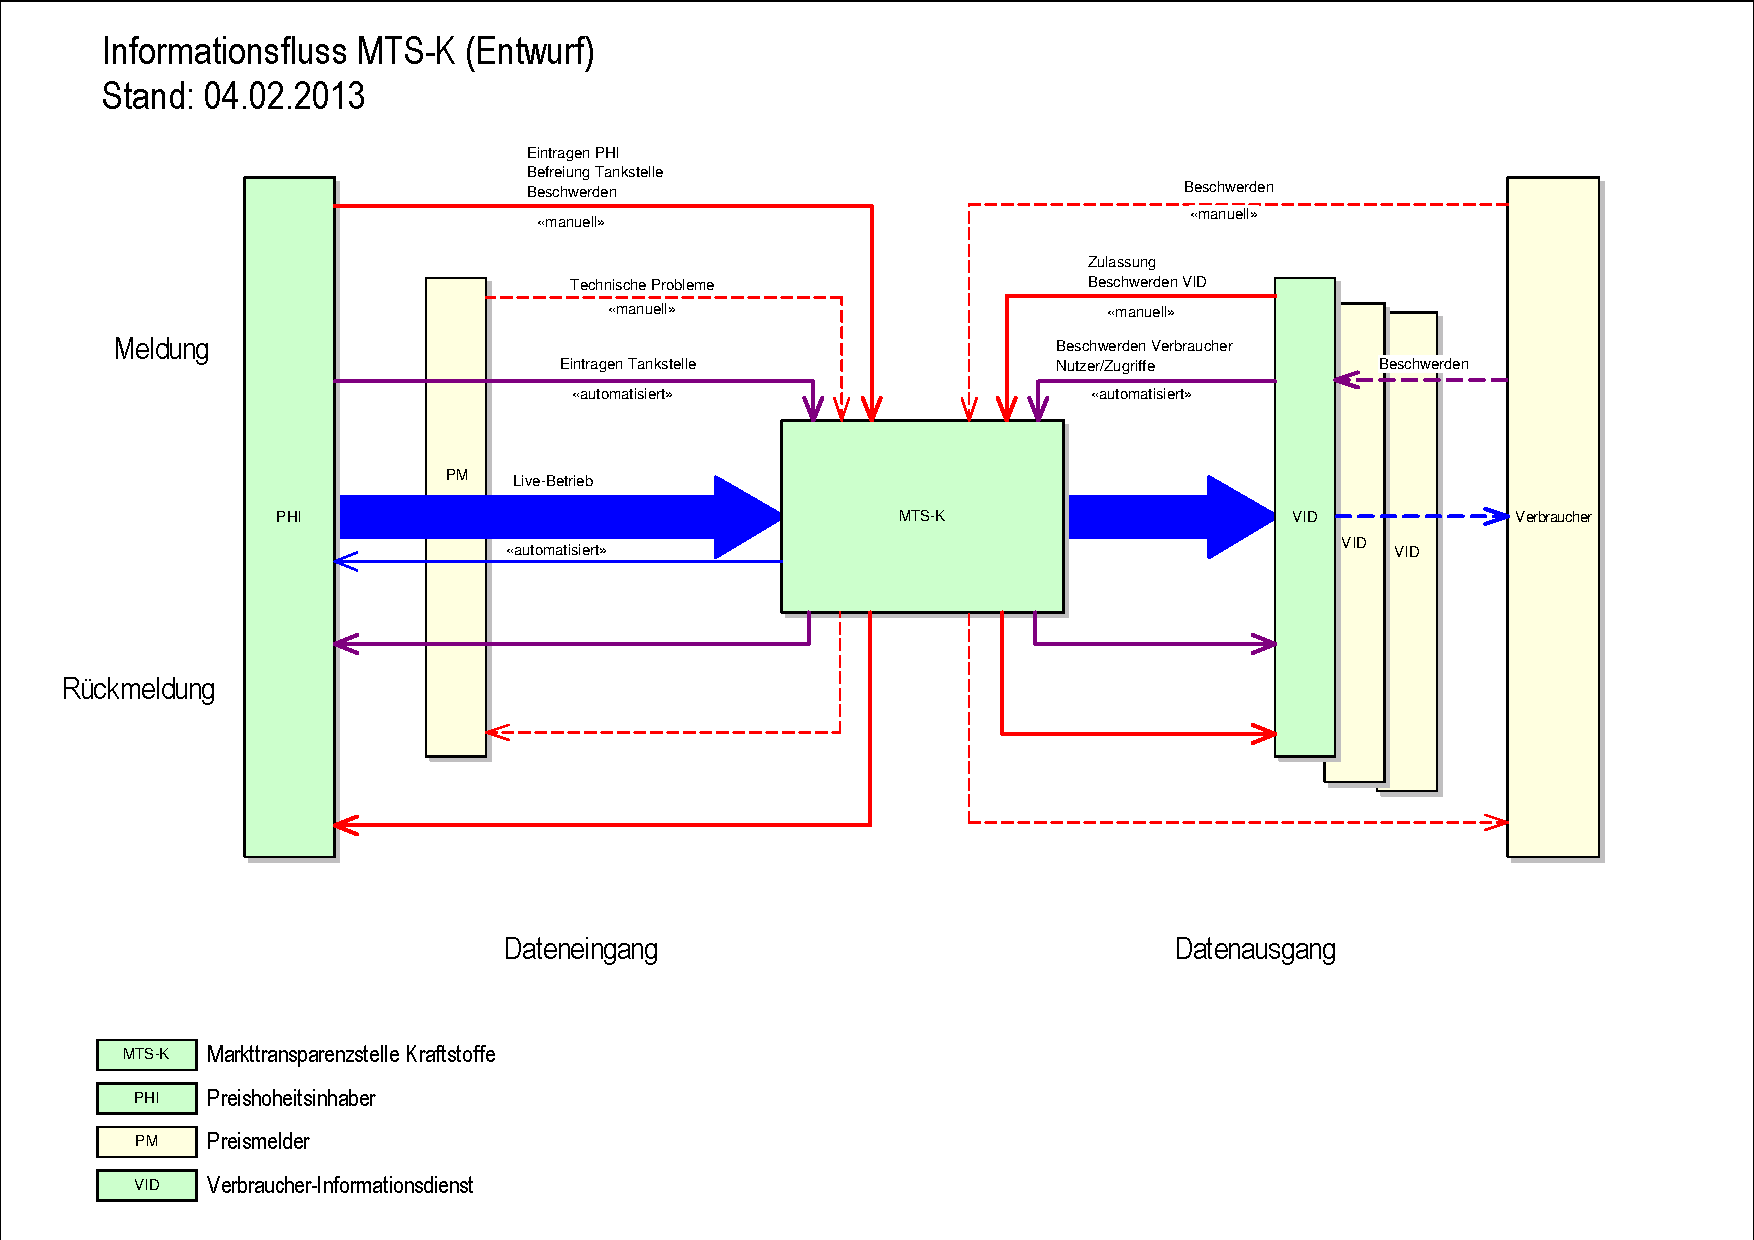
\includegraphics[width=0.8\textwidth]{Bilder/Informationsfluss-MTS.png}\\
	\captionof{figure}[MTS]{Informationsfluss der MTS-K\cite{IMTSK}}
	\label{fig:MTS-K}
\end{center} 

Die Daten für diese Arbeit entstammen dem Verbraucherinformationsdienst der Tankerkönig API. Tankerkönig bezieht seine Daten direkt von der MTS  und stellt diese sowohl im Zuge einer Echtzeit-Benzinpreis-API als auch gesondert aufbereitet als historische Datenbank in Form eines PostgreSQL dumps im 9.4.-Format zur Verfügung. Die für diese Arbeit verwendeten dumps umfassen neben den kompletten Preisedaten vom 8.6.2014 bis zum 2.5.2016 auch die Informationen über die Stammdaten der Tankstellen.\cite{TkAPI} 

\begin{center}
	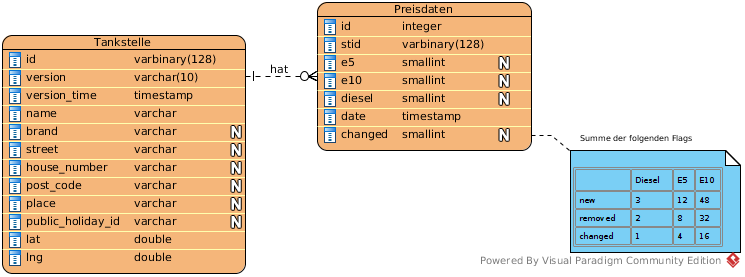
\includegraphics[width=0.8\textwidth]{Bilder/pricing_data.png}\\
	\captionof{figure}[ERD Tankerkönig]{ERD des historischen Datensatzes}
	\label{fig:ERD-T}
\end{center}

\titlespacing{\subsection}{0pt}{12pt plus 4pt minus 2pt}{-6pt plus 2pt minus 2pt}
\subsection{Pricing-Tools}

Besonders hilfreich sind die Daten der MTS für Kraftstoffe natürlich für die Tanstellen selber. Die Live- Verfügbarkeit aller momentanen Preise macht das konkurieren mit anderen Tankstellen viel einfacher und schneller. Verbunden mit der Homogenität des Produktes ermöglicht es diese neuartige technische Informationsquelle Preise vollautomatisch und gleichzeitig konkurenzfähig anpassen zu lassen, da der für den Kunden einzig interessante Aspekt an dem Produkt der niedrigste Preis ist. Im Zuge dessen sind einige Pricing-Tools enstanden um das hochfrequente Preise wechseln einfacher zu gestalten. Während mittelständische Unternehmen auf externe Software Solutions zurückgreifen, so wie zum Beispiel die Q1 und Westfalen AG auf Angebote der Firmen Temiz4u\footnotemark[1] und Weat\footnotemark[2], ist es anzunehmen, dass die großen fünf der Szene Aral, Shell, Jet, Esso und Total ihre eigenen internen Programme verwenden werden. Im Verlauf dieses Abschnittes soll am Beispiel so eines Tools herausgestellt werden, was für Einstellungsmöglichkeiten der Nutzer bei den Regeln in so einem Tool hat, da all diese später als Parameter in den zu erkennenden Mustern auftreten werden. Die drei groben Teilaspekte, Konkurenzbereich, Regelsetzung und Automatisierungsgrad, die sich hier bei der Untergliederung ergeben, werden dementsprechen auch in der im nächsten Kapitel folgenden Zielsetzung vorzufinden sein. Die hier vorgestellt Funktionsweise beschreibt ein rein reaktives, das heißt es reagiert auf Preisänderungen anderer Tankstellen und wird nicht von sich aus Preise aktive ändern.

\footnotetext[1]{Quelle: \url{https://www.temiz4u.net/web/guest/solutions}}
\footnotetext[2]{Quelle: \url{http://www.weat.de/produkte/pricing/}}

\titlespacing{\subsubsection}{0pt}{12pt plus 4pt minus 2pt}{-6pt plus 2pt minus 2pt}
\subsubsection{Generelle Funktionsweise}
Würde das Programm immer vollautomatisch laufen und nicht anhalten, wäre es im Grunde ähnlich zu einem $\omega$ -Automat, oder auch unendlichen Automat. Die Definition so eines Automaten besteht ähnlich den endlichen Automaten aus einem 5-Tupel:
\begin{enumerate}
\item dem endlichen Eingabealphabet
\item der endlichen Zustandsmenge
\item einem Startzustand
\item einem Übergangsalphabet
\item einer Menge an akzeptieren Zuständen die hier ganz verschieden aussehen können
\end{enumerate}

Bezogen auf unseren Kontext wären der generelle Marktzustand zu einem bestimmten Zeitpunkt, insbesondere der Preisstand der eigenen Tankstelle und der Zeitpunkt an sich die Komponenten der Zustandsmenge also insbesondere auch des Startzustandes und der akzeptierenden Zustände.
Die Übergangsfunktion wird über bestimmte Regeln definiert, also wie auf welche Preisänderungen zu welchem Zeitpunkt reagiert werden soll. Die Festlegung der Endzustände ist nicht ganz trivial, da das Programm unendlich lange laufen soll. Man könnte bestimmte Zeitpunkte festlegen ab dem sich die festgelegten Regeln wiederholen zum Beispiel nach einem Tag, einer Woche oder einem Jahr, ganz abhängig von den hinterlegten Regeln.Ein großes Problem in der Praxis ist, wie später noch ausführlich diskutiert werden wird, dass die Regeln beliebig geändert werden können es also keine wiederkehrenden Muster geben muss beziehungsweise der Automat für beliebige Zeit sogar abgeschaltet werden kann.

\titlespacing{\subsubsection}{0pt}{12pt plus 4pt minus 2pt}{-6pt plus 2pt minus 2pt}
\subsubsection{Einstellungsoptionen für Regeln}
\textcolor{red}{Die Bilder für diese Sektion müssen eventuell noch einmal überarbeitet werden weil sie eventuell vertrauliche Informationen enthalten}\\
Die Einstellungsoptionen lassen sich grob in drei größere Kategorien unterteilen, welche auch später wieder bei der Untergliederung der Zielsetzung eine Rolle spielen werden.
\begin{enumerate}
\item[a)] Konkurenz Bestimmung:\\ 

\begin{center}
	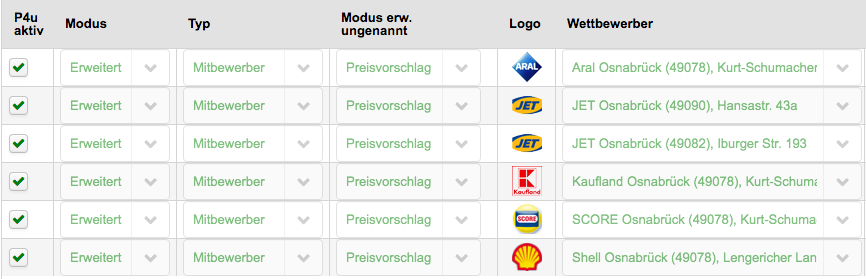
\includegraphics[width=0.8\textwidth, draft]{Bilder/konkurenz.png}\\
	\captionof{figure}[PT-K]{Princing Tool Konkurenz Bestimmung}
	\label{fig:PT-K}
\end{center}
Hier wird eine Liste von Tankstellen eingestellt, die als Konkurenten erachtet werden. Diese sowie auch noch später folgende Einstellungen sind sozusagen eine Art Filterfunktion für die Zustandsübergänge. Nur Preisänderungen von diesen Tankstellen sind interessant und erfordern wohlmöglich eine Reaktion.

\item[b)] Regel Festlegung:\\
\begin{center}
	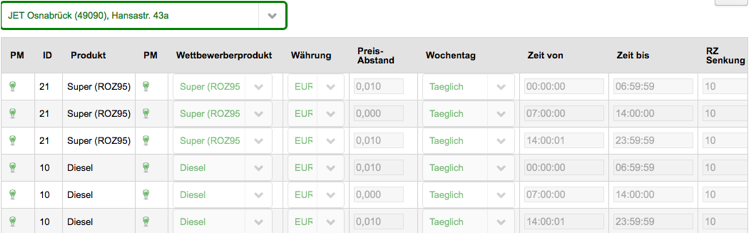
\includegraphics[width=0.8\textwidth, draft]{Bilder/regeln2.png}\\
	\captionof{figure}[PT-R]{Princing Tool Regel Festlegung}
	\label{fig:PT-R}
\end{center}
Das Kernstück dieser Tools und der Grund, warum das Erkennen von Mustern so schwierig ist, sind die Regeln und deren Variabilität. Für jeden Konkurenten kann ein eigenes Regelwerk angelegt werden. Jede Regel beschreibt in welchem Zeitfenster welcher preisliche Abstand zu dem jeweiligen Konkurenten bestehen soll, und nach wie vielen Minuten Verzögerung dieser bei Abweichung wiederhergestellt werden soll. Besonders Variable ist hier das Zeitintervall, welches theoretisch für jeden Wochentag beliebig gewählt werden kann.

\item[c)] Automatik Einstellung:\\
\begin{center}
	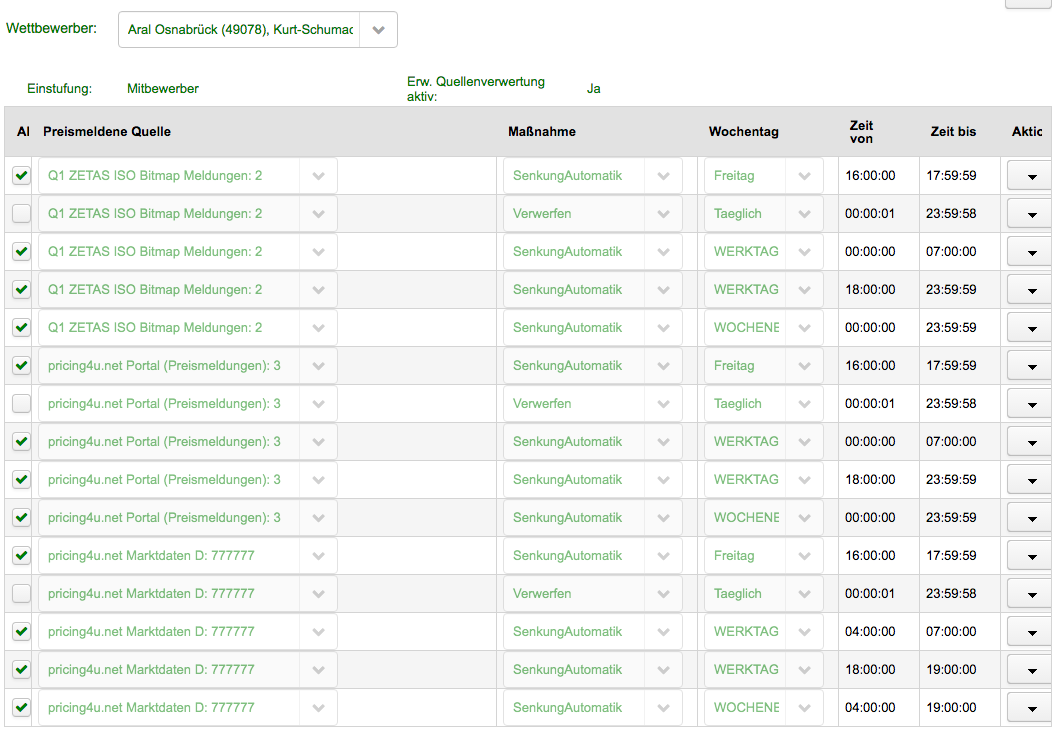
\includegraphics[width=0.8\textwidth, draft]{Bilder/automatik.png}\\
	\captionof{figure}[PT-A]{Princing Tool Automatik Einstellung}
	\label{fig:PT-A}
\end{center}
Das Tool bietet prinzipiell zwei verschiedene Modi an in denen der Nutzer das Pricing betreiben kann. Es kann entweder vollautomatisch arbeiten, das heißt nach den definierten Regeln die Preisänderungen selber direkt vornehmen. Oder es erteilt basierend auf den Regeln Preisänderungsvorschläge, die dann vom Nutzer nach eigenem Ermessen durchgeführt werden können der nicht, wobei die Verzögerungszeit in diesem Fall womöglich von der Reaktionszeit des Nutzers abhängt. Wie auch schon bei den Regeln kann hier für jeden Wochentag für jedes beliebige Zeitintervall eingestellt werden, welcher Modus praktiziert werden soll.
\end{enumerate}



% \titlespacing{\subsection}{0pt}{12pt plus 4pt minus 2pt}{-6pt plus 2pt minus 2pt}
% \subsection{Hintergrundwissen und Strategien im Pricing Verhalten}

% \titlespacing{\section}{0pt}{12pt plus 4pt minus 2pt}{-6pt plus 2pt minus 2pt}
% \section{Stand der Technik}

% \vspace{-1,2em}

\vspace{-1,2em}
\newpage

% \titlespacing{\section}{0pt}{12pt plus 4pt minus 2pt}{-6pt plus 2pt minus 2pt}
% \section{Anforderungsanalyse}
\titlespacing{\section}{0pt}{12pt plus 4pt minus 2pt}{-6pt plus 2pt minus 2pt}
\section{Zielsetzung}
Thema dieses Abschnittes ist es das Ziel oder die Ziele dieser Arbeit weiter aufzugliedern und so genau wie möglich zu spezifizieren. Dabei werden möglicherweise auftretende Probleme, die sich aus den Arbeitsgrundlagen ergeben könnten, angesprochen und etwaige Lösungsansätze diskutieren. Die Zielsetzung Verhaltensmuster im Pricing von Tankstellen zu erkennen ist bei einer Menge von ca 65 Millionen Preisänderugen zu grob und unhandlich. Es sollte zunächst genauer eingeschränkt werden in welchen Teilbereichen überhaupt Muster vermutet werden, um den Suchbereich zu minimieren. In diesem Fall bedeutet das herauszufinden, welche Tankstellen untereinander aufeinander reagieren also sich als Konkurenz betrachten. Unter den konkurierenden Tankstellen gilt es nun herauszufinden, ob bzw. in welchem Maße das Reaktionsverhalten automatisert geregelt zu sein scheint und die zu Grunde liegenden Regeln zurückzuverfolgen. Des weiteren könnte man untersuchen in welchem Ausmaß sich Konkurenzbereiche  untereinander verketten und somit eventuell größere Preissektoren bilden. Letztlich wäre es noch interessant herauszufinden, ob es Tankstellen gibt die regelmäßig Preissenkungen auslösen sprich ob sich Akteure und Reakteure spezifizieren lassen, oder ob vielleicht alle Senkungen zyklische Reaktionen auf unterschiedlich hohe Preiserhöhungen sind.

\titlespacing{\subsection}{0pt}{12pt plus 4pt minus 2pt}{-6pt plus 2pt minus 2pt}
\subsection{Konkurenten erkennen}

Konkurierende Tankstellen sind Tankstellen mit einem potentiell gleichen Klientel. Das bedeuted, da Kraftstoff immernoch vor Ort gekauft und getankt wird, dass in erster Linie räumliche Nähe das ausschlaggebenste Kriterium ist, um Konkurenz zu bestimmen. Jeder Tankstelle kann also zunächst mittels einer Abstandstandsbestimmung über die Geolocations ein potentieller Konkurentenkreis zugewiesen werden.\\

Ein erstes Problem bildet hier die Festlegung eines oberen Abstands-Thresholds, um die Anzahl der potentiellen KOnkurenten, welche es zu überprüfen gilt, möglichst gering zu halten. Die kritische Nähe ist hierbei stark an den Besiedelungsgrad der unmittelbaren Umgebung gebunden. So kann es in der Stadt durchaus sein, dass der nächste Konkurent auf der anderen Straßenseite zu finden ist und sich noch 15 oder mehr weitere Tankstellen im Umkreis von wenigen Kilometern befinden, wohingegen es beispielsweise auf der Autobahn vorkommen kann, dass die nächste Tankstelle mehr als 10km entfernt liegt. Eine harte obere Schranke wäre hier nicht besonders zielführend. Andererseits scheint es intuitiv plausibel, dass die Anzahl an Konkurenten beschränkt sein sollte. Man könnte also die Anzahl sowohl nach unten als auch nach oben beschränken und von einem geringen Abstand startend den Abstand iterativ erhöhen, wenn nötig.\\

Obwohl der Abstand nicht das einzige oder auch ökonomisch sinnvollste Kriterium darstellt, so ist es doch das intuitivste und informationstechnisch am einfachsten auszuwertende. Viel aussagekräftiger wäre eigentlich die Schnittmenge des Verkehrsflusses. Die gegenüberliegende Tankstelle auf der Autobahn ist zwar räumlich nicht gerade  weit entfent, für die Verkehrsteilnehmer aber nur über einen erheblichen Umweg zu erreichen. Ähnliches gilt auch für verschiedene Hauptverkehrsstraßen in Städten. Unter Umständen könnte auch die Uhrzeit relevant sein, wenn man beispielsweise das Pendlerverhalten als weiteres Kriterium hinzunimmt. Man könnte zwar versuchen über Navigationsprogramme und Verkehrflussanalysen zu einer ökonomisch genaueren Auswahl zu kommen, jedoch steht der Aufwand hierfür in keinem Verhältnis zum potentiellen Gewinn. Ziel dieses Abschnittes ist es letztlich ja auch nicht die sinnvollsten Konkurenten zu ermitteln, sondern jene die sich wie Konkurenten verhalten. Da auch nicht ohne weiteres davon ausgegangen werden kann, dass jede Tankstelle ihre Konkurenz ökonomisch korrekt ermittelt hat, ist es zunächst ausreichend eine grobe Auswahl zu treffen, da die wahre Konkurenz im nächsten Schritt über die Analyse des Pricingverhaltens bestimmt wird.\\

Um nun aus dem Kreis der potentiellen Konkurenten die wahren Konkurenten zu extrahieren müssen im Pricingverhalten Parameter gefunden werden die nahe legen, dass eine Preisänderung eine Reaktion auf den Preis bzw die Preisänderung einer benachbarten Tankstelle ist, die beiden Tankstellen also in einer Art kausalen Relation stehen. Abgesehen davon, dass hier insbesondere auf die Möglichkeiten eingegangen werden sollte, die die Pricing-Tools zur automatisierten Reaktion bereitstellen, ist der wohl wichtigste Parameter in Sachen Kausalität immernoch die zeitliche Nähe. So hochfrequent, wie sich die Preise in diesem Bereich inzwischen ändern, wäre mehr als eine Stunde Verzögerung wohl kaum noch als Reaktion aufzufassen. Andererseits bereitet diese hohe Frequenz zusammen mit doch üblichen, da auch gewollten, Verzögerungen von mehr als 10 Minuten auch Probleme, wenn bei mehreren zeitlich korrelierenden Veränderungen nicht mehr ersichtlich ist, welche letztlich auch kausal verantwortlich war. Die Analyse von Korrelationen und Kausalität in Zeitreihendaten ist ein weit verbreitetes Problem und daher relativ ausgiebig erforschtes Gebiet mit etlichen Algorithmen und ihren Variationen, ganz vorne an der Granger Kausality Test, welche auf ihre Anwendbarkeit in diesem Szenario hin untersucht werden können.\\

Zusätzlich gibt es noch ein paar andere logische Zusammenhänge, die man als Parameter heranziehen könnte. Konkurenz ist nicht immer aber in aller Regel eine Wechselseitige Beziehung. Es liegt also nahe, dass, wo in einer Richtung konkurierendes Verhalten festgestellt wurde, ähnliches auch in die andere Richtung zu vermuten ist. Demnach sollte es auch einen zeitlich relativ stabilen Preisabstand zwischen zwei Konkurenten geben, der bei einer Preisänderung gebrochen wird. Wäre dem nicht so und hätten zwei konkurierende Tankstellen in ihren Tools zwei miteinander nicht konsistente gewünschte Preisabstände zum jeweilig Anderen in ihren Regeln hinterlegt, dann würde bei einer automatischen Betreibung des Pricings der Preis innerhalb kürzester Zeit auf das festgelegt Minimum herabfallen, was auf keinen Fall im Interesse beider Tankstellen sein kann. Die Preisänderung, die den Bruch dieses Abstandes herbeiführt, muss also durch die Reaktion auf einen anderen Konkurenten enstanden sein. Die reagierende Preisänderung sollte demnach nur diesen stabilen Abstand wieder herbeiführen.

\titlespacing{\subsection}{0pt}{12pt plus 4pt minus 2pt}{-6pt plus 2pt minus 2pt}
\subsection{Automatisierungsgrad bestimmen}

\titlespacing{\subsection}{0pt}{12pt plus 4pt minus 2pt}{-6pt plus 2pt minus 2pt}
\subsection{Regeln spezifizieren}

\titlespacing{\subsection}{0pt}{12pt plus 4pt minus 2pt}{-6pt plus 2pt minus 2pt}
\subsection{Kettenbildung untersuchen}

\titlespacing{\subsection}{0pt}{12pt plus 4pt minus 2pt}{-6pt plus 2pt minus 2pt}
\subsection{Unterscheidung zwischen Akteur und Reakteur}

\pagebreak

% % ----------------------------------------------------------------------------------------------------------
% % Verzeichnisse
% % ----------------------------------------------------------------------------------------------------------
% % TODO Typ vor Nummer
% \renewcommand{\cfttabpresnum}{Tab. }
% \renewcommand{\cftfigpresnum}{Abb. }
% \settowidth{\cfttabnumwidth}{Abb. 10\quad}
% \settowidth{\cftfignumwidth}{Abb. 10\quad}

% \titlespacing{\section}{0pt}{12pt plus 4pt minus 2pt}{2pt plus 2pt minus 2pt}
% \singlespacing
% \rhead{INHALTSVERZEICHNIS}
% \renewcommand{\contentsname}{II Inhaltsverzeichnis}
% \phantomsection
% \addcontentsline{toc}{section}{\texorpdfstring{II \hspace{0.35em}Inhaltsverzeichnis}{Inhaltsverzeichnis}}
% \addtocounter{section}{1}
% \tableofcontents
% \pagebreak
% \rhead{VERZEICHNISSE}
% \listoffigures
% \pagebreak
% \listoftables
% %\pagebreak
% \renewcommand{\lstlistlistingname}{Listing-Verzeichnis}
% {\labelsep2cm\lstlistoflistings}
% \pagebreak

% % ----------------------------------------------------------------------------------------------------------
% % Abkürzungen
% % ----------------------------------------------------------------------------------------------------------
% \section{Abkürzungsverzeichnis}
% \begin{acronym}[OSGi] % längste Abkürzung steht in eckigen Klammern
% 	\setlength{\itemsep}{-\parsep} % geringerer Zeilenabstand
% 	\acro{OSGi}{Open Service Gateway initiative}
% \end{acronym}
% \newpage

% % ----------------------------------------------------------------------------------------------------------
% % Inhalt
% % ----------------------------------------------------------------------------------------------------------
% % Abstände Überschrift
% \titlespacing{\section}{0pt}{12pt plus 4pt minus 2pt}{-6pt plus 2pt minus 2pt}
% \titlespacing{\subsection}{0pt}{12pt plus 4pt minus 2pt}{-6pt plus 2pt minus 2pt}
% \titlespacing{\subsubsection}{0pt}{12pt plus 4pt minus 2pt}{-6pt plus 2pt minus 2pt}

% % Kopfzeile
% \renewcommand{\sectionmark}[1]{\markright{#1}}
% \renewcommand{\subsectionmark}[1]{}
% \renewcommand{\subsubsectionmark}[1]{}
% \lhead{Kapitel \thesection}
% \rhead{\rightmark}

% \onehalfspacing
% \renewcommand{\thesection}{\arabic{section}}
% \renewcommand{\theHsection}{\arabic{section}}
% \setcounter{section}{0}
% \pagenumbering{arabic}
% \setcounter{page}{1}

% % ----------------------------------------------------------------------------------------------------------
% % Einleitung
% % ----------------------------------------------------------------------------------------------------------
% \section{Einleitung}
% Dieses Kapitel enthält Beispiele zum Einfügen von Abbildungen, Tabellen, etc.

% \subsection{Bilder}
% Zum Einfügen eines Bildes, siehe Abbildung \ref{fig:osgi}, wird die \textit{minipage}-Umgebung genutzt, da die Bilder so gut positioniert werden können.

% \vspace{1em}
% \begin{minipage}{\linewidth}
% 	\centering
% 	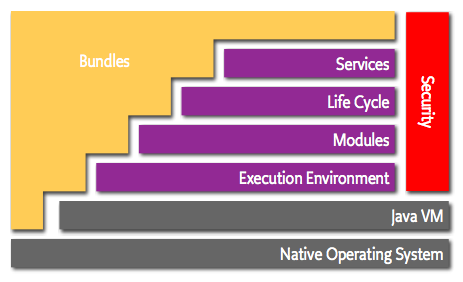
\includegraphics[width=0.7\linewidth]{Bilder/layering-osgi.png}
% 	\captionof{figure}[OSGi Architektur]{OSGi Architektur\footnotemark }
% 	\label{fig:osgi}
% \end{minipage}
% \footnotetext{Quelle: \url{http://www.osgi.org/Technology/WhatIsOSGi}}

% \subsection{Tabellen}
% In diesem Abschnitt wird eine Tabelle (siehe Tabelle \ref{tab:beispiel}) dargestellt.

% \vspace{1em}
% \begin{table}[!h]
% 	\centering
% 	\begin{tabular}{|l|l|l|}
% 		\hline
% 		\textbf{Name} & \textbf{Name} & \textbf{Name}\\
% 		\hline
% 		1 & 2 & 3\\
% 		\hline
% 		4 & 5 & 6\\
% 		\hline
% 		7 & 8 & 9\\
% 		\hline
% 	\end{tabular}
% 	\caption{Beispieltabelle}
% 	\label{tab:beispiel}
% \end{table}

% \pagebreak
% \subsection{Auflistung}
% Für Auflistungen wird die \textit{compactitem}-Umgebung genutzt, wodurch der Zeilenabstand zwischen den Punkten verringert wird.

% \begin{compactitem}
% 	\item Nur
% 	\item ein
% 	\item Beispiel.
% \end{compactitem}

% \subsection{Listings}
% Zuletzt ein Beispiel für ein Listing, in dem Quellcode eingebunden werden kann, siehe Listing \ref{lst:arduino}.

% \vspace{1em}
% \begin{lstlisting}[caption=Arduino Beispielprogramm, label=lst:arduino]
% int ledPin = 13;
% void setup() {
%     pinMode(ledPin, OUTPUT);
% }
% void loop() {
%     digitalWrite(ledPin, HIGH);
%     delay(500);
%     digitalWrite(ledPin, LOW);
%     delay(500);
% }
% \end{lstlisting}

% Die Quellen befinden sich in der Datei \textit{bibo.bib}. Ein Buch- und eine Online-Quelle sind beispielhaft eingefügt. [Vgl. \cite{buch}]

% Abkürzungen lassen sich natürlich auch nutzen (\ac{OSGi}). Weiter oben im Latex-Code findet sich das Verzeichnis.
% \pagebreak

% % ----------------------------------------------------------------------------------------------------------
% % Kapitel
% % ----------------------------------------------------------------------------------------------------------
% \section{Kapitel}
% Lorem ipsum dolor sit amet.

% \subsection{Unterkapitel}
% Lorem ipsum dolor sit amet, consetetur sadipscing elitr, sed diam nonumy eirmod tempor invidunt ut labore et dolore magna aliquyam erat, sed diam voluptua. At vero eos et accusam et justo duo dolores et ea rebum. Stet clita kasd gubergren, no sea takimata sanctus est Lorem ipsum dolor sit amet. Lorem ipsum dolor sit amet, consetetur sadipscing elitr, sed diam nonumy eirmod tempor invidunt ut labore et dolore magna aliquyam erat, sed diam voluptua. At vero eos et accusam et justo duo dolores et ea rebum. Stet clita kasd gubergren, no sea takimata sanctus est Lorem ipsum dolor sit amet.

% \subsection{Unterkapitel}
% Lorem ipsum dolor sit amet, consetetur sadipscing elitr, sed diam nonumy eirmod tempor invidunt ut labore et dolore magna aliquyam erat, sed diam voluptua. At vero eos et accusam et justo duo dolores et ea rebum. Stet clita kasd gubergren, no sea takimata sanctus est Lorem ipsum dolor sit amet. Lorem ipsum dolor sit amet, consetetur sadipscing elitr, sed diam nonumy eirmod tempor invidunt ut labore et dolore magna aliquyam erat, sed diam voluptua. At vero eos et accusam et justo duo dolores et ea rebum. Stet clita kasd gubergren, no sea takimata sanctus est Lorem ipsum dolor sit amet.
% \pagebreak

% % ----------------------------------------------------------------------------------------------------------
% % Kapitel
% % ----------------------------------------------------------------------------------------------------------
% \section{Kapitel}
% Lorem ipsum dolor sit amet.

% \subsection{Unterkapitel}
% Lorem ipsum dolor sit amet, consetetur sadipscing elitr, sed diam nonumy eirmod tempor invidunt ut labore et dolore magna aliquyam erat, sed diam voluptua. At vero eos et accusam et justo duo dolores et ea rebum. Stet clita kasd gubergren, no sea takimata sanctus est Lorem ipsum dolor sit amet. Lorem ipsum dolor sit amet, consetetur sadipscing elitr, sed diam nonumy eirmod tempor invidunt ut labore et dolore magna aliquyam erat, sed diam voluptua. At vero eos et accusam et justo duo dolores et ea rebum. Stet clita kasd gubergren, no sea takimata sanctus est Lorem ipsum dolor sit amet.

% \subsection{Unterkapitel}
% Lorem ipsum dolor sit amet, consetetur sadipscing elitr, sed diam nonumy eirmod tempor invidunt ut labore et dolore magna aliquyam erat, sed diam voluptua. At vero eos et accusam et justo duo dolores et ea rebum. Stet clita kasd gubergren, no sea takimata sanctus est Lorem ipsum dolor sit amet. Lorem ipsum dolor sit amet, consetetur sadipscing elitr, sed diam nonumy eirmod tempor invidunt ut labore et dolore magna aliquyam erat, sed diam voluptua. At vero eos et accusam et justo duo dolores et ea rebum. Stet clita kasd gubergren, no sea takimata sanctus est Lorem ipsum dolor sit amet.
% \pagebreak

% % ----------------------------------------------------------------------------------------------------------
% % Kapitel
% % ----------------------------------------------------------------------------------------------------------
% \section{Kapitel}
% Lorem ipsum dolor sit amet.

% \subsection{Unterkapitel}
% Lorem ipsum dolor sit amet, consetetur sadipscing elitr, sed diam nonumy eirmod tempor invidunt ut labore et dolore magna aliquyam erat, sed diam voluptua. At vero eos et accusam et justo duo dolores et ea rebum. Stet clita kasd gubergren, no sea takimata sanctus est Lorem ipsum dolor sit amet. Lorem ipsum dolor sit amet, consetetur sadipscing elitr, sed diam nonumy eirmod tempor invidunt ut labore et dolore magna aliquyam erat, sed diam voluptua. At vero eos et accusam et justo duo dolores et ea rebum. Stet clita kasd gubergren, no sea takimata sanctus est Lorem ipsum dolor sit amet.

% \subsection{Unterkapitel}
% Lorem ipsum dolor sit amet, consetetur sadipscing elitr, sed diam nonumy eirmod tempor invidunt ut labore et dolore magna aliquyam erat, sed diam voluptua. At vero eos et accusam et justo duo dolores et ea rebum. Stet clita kasd gubergren, no sea takimata sanctus est Lorem ipsum dolor sit amet. Lorem ipsum dolor sit amet, consetetur sadipscing elitr, sed diam nonumy eirmod tempor invidunt ut labore et dolore magna aliquyam erat, sed diam voluptua. At vero eos et accusam et justo duo dolores et ea rebum. Stet clita kasd gubergren, no sea takimata sanctus est Lorem ipsum dolor sit amet.
% \pagebreak

% ----------------------------------------------------------------------------------------------------------
% Literatur
% ----------------------------------------------------------------------------------------------------------
\renewcommand\refname{Quellenverzeichnis}
\bibliographystyle{myalpha}
\bibliography{bibo}
\pagebreak

% % ----------------------------------------------------------------------------------------------------------
% % Anhang
% % ----------------------------------------------------------------------------------------------------------
% \pagenumbering{Roman}
% \setcounter{page}{1}
% \lhead{Anhang \thesection}

% \begin{appendix}
% \section*{Anhang}
% \phantomsection
% \addcontentsline{toc}{section}{Anhang}
% \addtocontents{toc}{\vspace{-0.5em}}

% \section{GUI}
% Ein toller Anhang.

% \subsection*{Screenshot}
% \label{app:screenshot}
% Unterkategorie, die nicht im Inhaltsverzeichnis auftaucht.

% \end{appendix}


% \newpage
% \thispagestyle{empty}
% \begin{center}
% 	\vspace*{5em}
% 	\huge\textbf{Erklärung}\\
% \end{center}
% \vspace{2em}
% Hiermit versichere ich, dass ich meine Abschlussarbeit selbständig verfasst und keine anderen als die angegebenen Quellen und Hilfsmittel benutzt habe.

% \vspace{4em}
% \begin{minipage}{\linewidth}
% 	\begin{tabular}{p{15em}p{15em}}
% 		Datum: &  .......................................................\\
% 		& \centering (Unterschrift)\\
% 	\end{tabular}
% \end{minipage}

\end{document}
